\documentclass[12pt]{article}
\usepackage{epsf}
\usepackage{amssymb}
\usepackage{enumitem}
\usepackage{amsmath}
\usepackage{tikz}
\usetikzlibrary{automata, positioning, arrows}

\title{aashlock-331-hw9}
\author{Aren Ashlock}
\date{March 28, 2024}

\setlength{\oddsidemargin}{-0.25in}
\setlength{\topmargin}{-0.5in}
\setlength{\headheight}{0cm}
\setlength{\headsep}{0cm}
\setlength{\textheight}{10in}
\setlength{\textwidth}{7in}
\setlength{\topskip}{0cm}

\begin{document}

\noindent\textbf{ComS 331 \quad Spring 2024 \quad Name: Aren Ashlock}

\begin{enumerate}

%----------------------------------- Q1 DONE -----------------------------------

\item Specify in detail a (deterministic) Turing machine that accepts the language $L$ of even-length palindromes over $\{a,b\}$ (your Turing machine must halt on input $w$ if, and only if, $w \in L$).

You must represent the TM as a graph showing the initial state (as we do in a DFA) and labeling the edges with the corresponding transition: for example, if $\delta(s,a) = (t,b)$, or $(t,L)$, or $(t,R)$, then label the edge from $s$ to $t$ with "$a,b$", or "$a,L$", or "$a,R$", respectively.

Remember: your machine is deterministic, so it must have a well-defined behavior for each input symbol, i.e, $a$, $b$, and \#, and each state (other than the halting state $h$).

\begin{tikzpicture}
    [node distance = 3cm]
    \node[state, initial, initial text=] (sA) {A};
    \node[state, right of = sA] (sB) {B};
    \node[state, right of = sB] (sH) {h};
    % added states
    \node[state, below of = sA] (sJ) {J};
    \node[state, below of = sH] (sK) {K};
    % ------------
    \node[state, below of = sJ] (sC) {C};
    \node[state, below of = sK] (sD) {D};
    \node[state, below of = sC] (sE) {E};
    \node[state, below of = sD] (sF) {F};
    \node[state, right of = sJ] (sG) {G};
    \node[state, right of = sE] (sI) {I};
    % added states
    \node[state, below of = sG] (sL) {L};
    % ------------

    \path[->] (sA) edge [loop, out=68, in=113, looseness=5, above] node {$a,R$; $b,R$} (sA);
    \path[->] (sA) edge [midway, above] node {$\#,L$} (sB);
    \path[->] (sB) edge [midway, above] node {$\#,\#$} (sH);
    \path[->] (sB) edge [midway, left] node {$a,\#$} (sJ);
    \path[->] (sB) edge [midway, right, bend left = 20] node {$b,\#$} (sK);
    % added paths
    \path[->] (sJ) edge [midway, left] node {$\#,L$} (sC);
    \path[->] (sK) edge [midway, right] node {$\#,L$} (sD);
    \path[->] (sJ) edge [loop, out=158, in=203, looseness=5, left] node {$a,a$; $b,b$} (sJ);
    \path[->] (sK) edge [loop, out=338, in=13, looseness=5, right] node {$a,a$; $b,b$} (sK);
    % -----------
    \path[->] (sC) edge [loop, out=158, in=203, looseness=5, left] node {$a,L$; $b,L$} (sC);
    \path[->] (sD) edge [loop, out=338, in=13, looseness=5, right] node {$a,L$; $b,L$} (sD);
    \path[->] (sC) edge [midway, left] node {$\#,R$} (sE);
    \path[->] (sD) edge [midway, right] node {$\#,R$} (sF);
    \path[->] (sE) edge [midway, left] node {$a,\#$} (sL);
    \path[->] (sF) edge [midway, right] node {$b,\#$} (sL);
    % added path
    \path[->] (sL) edge [midway, right] node {$\#,R$} (sG);
    \path[->] (sL) edge [loop, out=248, in=293, looseness=5, below] node {$a,a$; $b,b$} (sL);
    % ----------
    \path[->] (sG) edge [midway, left] node {$\#,L$} (sB);
    \path[->] (sG) edge [loop, out=30, in=75, looseness=5, below right] node {$a,R$; $b,R$} (sG);
    \path[->] (sE) edge [midway, below] node {$b,\#$; $\#,\#$} (sI);
    \path[->] (sF) edge [midway, below] node {$a,\#$; $\#,\#$} (sI);
    \path[->] (sI) edge [loop, out=248, in=293, looseness=5, below] node {$a,\#$; $b,\#$; $\#,\#$} (sI);
\end{tikzpicture}

%-------------------------------------------------------------------------------

\end{enumerate}
\end{document}